\subsection{Implementation}

Formålet med dette afsnit er at give en beskrivelse af programmets opbygning og struktur, samt ved brug af kodeeksempler at illustrere hvordan der gøres brug af den tidligere beskrevet teori til at lave programmet. I afsnittet vil der kun fremgå udvalgte kodeeksempler, men hele programmet kan findes i bilag. 

\subsubsection{Programbeskrivelse}

Programmet er udarbejdet som et suplement til hjemmesider som sælger lamper. Formålet med programmet er at hjælpe kunderne med at visualisere lampers belysning. Programmet har fokus på realitsk visualisering af lys fra lamper, samt muligheden for at ændre pærens farvetemperatur og synsvinkel.
Nedenstående figur viser et billede af renderingen fra det færdige program

[Indsæt rendering fra det færdige program]()
[nærmere beskrivelse af billede]()


\subsubsection{Programmets opbygning}

Programmet er opbygget efter desginprincippet "top-down programmering". Princippet går ud på at dele programmet og i mindre dele, og derefter løse de mindre dele i hver deres funktion. Funktionerne samles i main, som kun bruges til kommunikation med brugeren. 
\ref{fig:topdown} viser tankegangen bag top-down programmering, hvor de enkelte problemer deles op og løses som delproblemer. 

\begin{figure}[H]
    \centering
    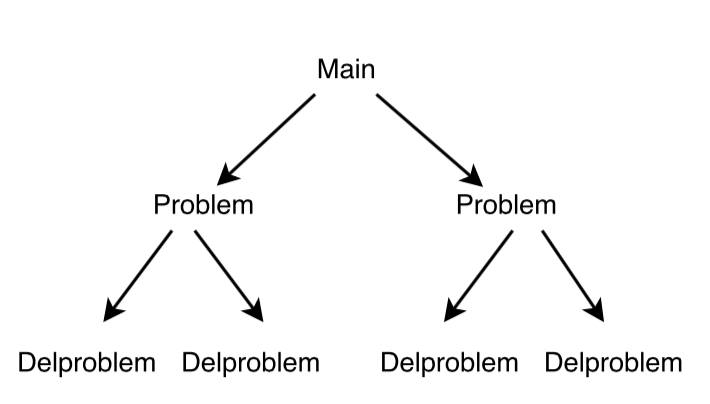
\includegraphics[width=10cm]{topdown}
    \caption{Tankegangen bag top-down programmering.}
    \label{fig:topdown}
\end{figure}

Som en del af vores top-down fremgangsmåde har vi struktureret opgaven i header-filer som blandt andet indeholder prototyper og structs. Header-filerne hjælper os med, at få bedre overblik over koden. 


\subsubsection{Vektorregning}
En vigtig del af vores raytracer består af vektorregning. For at regne med vektorer har vi valgt at bruge en struct for at abstrahere over vektorer. Som angivet i programmet kan det ses at en vektor består af tre koordinater, x, y og z. 

\begin{lstlisting}[style=Cstyle, caption=Vektorprototyper og struct]
typedef struct _vector {
    double x,y,z;
} Vector;

Vector vector_add(Vector v1, Vector v2);
Vector vector_subtract(Vector v1, Vector v2);
Vector vector_scale(Vector v, double s);
double vector_dot(Vector v1, Vector v2);
double vector_norm(Vector v);
Vector vector_normalize(Vector v);
double vector_angle_between(Vector v1, Vector v2);
Vector vector_cross(Vector v1, Vector v2);
Vector vector_rotate_around_z(Vector v, double angle);
Vector vector_rotate_around_x(Vector v, double angle);

\end{lstlisting}

Et eksempel på én af vores vektorudregninger er vector\_add. Denne funktion adderer to vektorer, som det ses på (program nr bla). Her kan man se, at ved addition af to vektorer, adderer man x-koordinaterne med hinanden og det samme gælder for y- og z-koordinaterne. Resultatet vil også være en vektor.

\begin{lstlisting}[style=Cstyle, caption=vector add]
Vector vector_add(Vector v1, Vector v2) {
  return (Vector){v1.x + v2.x, v1.y + v2.y, v1.z + v2.z};
}

\end{lstlisting}

Et andet eksempel på en vektorudregning, vi gør brug af, er skalarproduktet af to vektorer. Det er vigtigt at kende skalarproduktet, da det benyttes i vector\_norm for at finde længden af to vektorer og i vector\_angle\_between for at finde vinklen mellem to vektorer. Herunder kan det ses, at skalarproduktet simpelt findes ved at gange de tilsvarende koordinater med hinanden.

\begin{lstlisting}[style=Cstyle, caption=vector dot]
double vector_dot (Vector v1, Vector v2) {
  return v1.x * v2.x + v1.y * v2.y + v1.z * v2.z;
}
\end{lstlisting}


Vores bibliotek til vektorregning indeholder funktioner til alle de almindelige vektoroperationer. 

\subsubsection{Pixels}
I programmet har vi valgt at indføre en algoritme, der kan ’oversætte’ en farvetemperatur, målt i kelvin, til en RGB-værdi (rød-, grøn-, blå-værdi), som tilsammen viser en bestemt farve. Dette program kan hjælpe kunden med at visualisere den farve, som en lampe vil udsende, da det er vigtigt hvilken farvetemperatur et lys fra en lampe har (se afsnit \ref{sec:lys} om lys). Algoritmen er lånt og oversat fra pseudokoden fra følgende hjemmeside \href{http://www.tannerhelland.com/4435/convert-temperature-rgb-algorithm-code/}{http://www.tannerhelland.com/} under afsnittet 'The Algorithm'. Algoritmen er lavet ud fra at plotte Charity’s original blackbody values, som kan findes her: \href{http://www.vendian.org/mncharity/dir3/blackbody/UnstableURLs/bbr_color.html}{http://www.vendian.org/}. Disse værdier rangerer fra 1.000 til 40.000 kelvin, og det er derfor ikke sikket, at værdier ude for disse grænser er ligeså præcise i overgangen fra farvetemperatur til RGB-værdi. Copyright m.m. mht. algoritmen står i selve programmet som en kommentar i delen ’pixel.c’.


For at beregne en farve af en pixel, er det først nødvendigt at lave en struct pixel, der fortæller programmet, hvad den består af. 
\begin{lstlisting}[style=Cstyle, caption=Struct af Pixel]
typedef struct _pixel {
  double red, green, blue;
} Pixel;
\end{lstlisting}

Herefter laves der funktionen create\_from\_color\_temperature(), som er af typen Pixel, og som tager en unsigned int kelvin som input. Ud fra de konklusioner, der blev omtalt i teoriafsnittet \ref{sec:temp_til_rgb}, som omhandlede konvertering fra farvetemperatur til RGB, har man ud fra da benyttede data kunne opstille nogle konklusioner, der har gjort algoritmen mere simpel. Det er derfor muligt at beregne en given farve på følgende måde: 
\begin{lstlisting}[style=Cstyle, caption=Beregning af rød farve]
if(kelvin <= 66){
  color.red = 255;
}
else{
  color.red = kelvin - 60;
  color.red = 329.698727446 * (pow(color.red, -0.1332047592));
  if(color.red < 0){
    color.red = 0;
  }
  if(color.red > 255){
    color.red = 255;
  }
}
\end{lstlisting}

Algoritmen benytter sig af konklusionen 'røde værdier under 6600 kelvin, er altid 255' fra afsnit \ref{sec:temptilrgb}. Grunden til at der står 66 og ikke 6600, er fordi programmet er indledt med at dividere kelvin-inputtet med 100. Længere i det nestede if-statement beregner programmet farven rød, vha. funktionen, som er lavet ud fra dataene, og der afsluttes med at sørge for, at hvis værdien overskrider maksimummet på 255, sættes det til at være lig med 255.


Her ses en liste over de resterende funktioner i pixel.c, og nedenunder forklares deres benyttelse:

\subparagraph{Liste af andre funktioner i pixel}
\begin{lstlisting}[style=Cstyle, caption=Andre funktioner i pixel]
Pixel create_pixel(double red, double green, double blue);
char pixel_component_to_byte(double);
Pixel pixel_scale(Pixel color, double scalar);
Pixel pixel_multiply(Pixel color1, Pixel color2);
Pixel pixel_add(Pixel color1, Pixel color2);
\end{lstlisting}

\begin{enumerate}

  \item create\_pixel - opretter en pixel af typen Pixel med en RGB-værdi.
  \item pixel\_component to byte – ændrer værdien af RGB fra at være mellem 0 og 1, til at være mellem 0 og 255.
  \item pixel\_scale - skalerer en given pixel.
  \item pixel\_multiply - ganger to pixels sammen, der bruges til colorblending og udregning af, hvor meget farve der optages 								  ift. intensitet.
  \item pixel\_add - adderer to pixels, for at kunne udregne gennemsnittet senere (eller hvad???????????). I denne funktion er 							 det vigtigt at den returnerede værdi ikke overskrider 1, hvilket er hvorfor vi har implementeret MIN, der 							 sørger for at returnere den mindste funktion, der er 1, hvis en farve overskrider 1. Funktionen kan ses her:
  
\lstinline$\#define MIN(a, b) ((a) < (b) ? (a) : (b))$  					

\end{enumerate}



\subsubsection{ray}
For at man kan arbejde med raytracing er man nødt til at konstruere rays. Dette gøres ved at lave en struct som indeholder rayens startpunkt beskrevet som en vektor, samt en direction beskrevet med en retningsvektor. 

\begin{lstlisting}[style=Cstyle, caption=ray funktioner og struct]
typedef struct _ray {
  Vector initial_point, direction;
} Ray;

Ray create_ray(Vector p1, Vector p2);
Vector ray_get_point(Ray ray, double t);
\end{lstlisting}

Nedenstående kode viser vores to ray funktioner, først create\_ray som returnerer en ray lavet ud fra en startvektor og en retningsvektor.\newline Ray\_get\_point skalerer vores retningsvektor op med en skaler, t, og adderer denne vektor med rayens startpunkt. Vi før nu en ny repræsentation af vores ray, som returneres i funktionen.

\begin{lstlisting}[style=Cstyle, caption=funktionerne create\_ray og ray\_get\_point]
Ray create_ray(Vector p1, Vector p2) {
  return (Ray){p1, vector_normalize(p2)};
}

Vector ray_get_point(Ray ray, double t) {
    return vector_add(ray.initial_point, vector_scale(ray.direction, t));
}
\end{lstlisting}

\subparagraph{Liste af funktioner i vektorregning}
\begin{enumerate}
  
  \item create\_ray laver en ray ud fra to vektorer
  \item ray\_get\_point skalerer rayens retningsvektor og adderer den med rayens startpunkt
  
\end{enumerate}


